%
% File acl2021.tex
%
%% Based on the style files for EMNLP 2020, which were
%% Based on the style files for ACL 2020, which were
%% Based on the style files for ACL 2018, NAACL 2018/19, which were
%% Based on the style files for ACL-2015, with some improvements
%%  taken from the NAACL-2016 style
%% Based on the style files for ACL-2014, which were, in turn,
%% based on ACL-2013, ACL-2012, ACL-2011, ACL-2010, ACL-IJCNLP-2009,
%% EACL-2009, IJCNLP-2008...
%% Based on the style files for EACL 2006 by 
%%e.agirre@ehu.es or Sergi.Balari@uab.es
%% and that of ACL 08 by Joakim Nivre and Noah Smith

\documentclass[11pt,a4paper]{article}
\usepackage[hyperref]{acl2021}
\usepackage{times}
\usepackage{latexsym}
\usepackage{amssymb}
\usepackage{amsmath}
\usepackage{graphicx}
\usepackage{enumitem}
\usepackage{comment}
\usepackage{array}
%\usepackage{booktabs}
\renewcommand{\UrlFont}{\ttfamily\small}

% This is not strictly necessary, and may be commented out,
% but it will improve the layout of the manuscript,
% and will typically save some space.
\usepackage{microtype}
\allowdisplaybreaks

\aclfinalcopy % Uncomment this line for the final submission
%\def\aclpaperid{***} %  Enter the acl Paper ID here

%\setlength\titlebox{5cm}
% You can expand the titlebox if you need extra space
% to show all the authors. Please do not make the titlebox
% smaller than 5cm (the original size); we will check this
% in the camera-ready version and ask you to change it back.

\newcommand\BibTeX{B\textsc{ib}\TeX}
\DeclareMathOperator*{\argmin}{arg\,min}

\title{Learn The Big Picture: Representation Learning for Clustering}

\author{Sumanta Kashyapi \\
  Department of Computer Science \\
  University of New Hampshire \\
  \texttt{sk1105@wildcats.unh.edu} \\\And
  Laura Dietz \\
  Department of Computer Science \\
  University of New Hampshire \\
  \texttt{dietz@cs.unh.edu} \\}

\date{}

\begin{document}
\maketitle
\begin{abstract}
Existing supervised models for text clustering find it difficult to directly optimize for clustering results. This is because clustering is a discrete process and it is difficult to estimate meaningful gradient of any discrete function that can drive gradient based optimization algorithms. So, existing supervised clustering algorithms indirectly optimize for some continuous function that approximates the clustering process. We propose a scalable training strategy that directly optimizes for a discrete clustering metric. We train a BERT-based embedding model using our method and evaluate it on two publicly available datasets. We show that our method outperforms another BERT-based embedding model employing Triplet loss and other unsupervised baselines. This suggests that optimizing directly for the clustering outcome indeed yields better representations suitable for clustering.
%Loss function based on this strategy is able to efficiently guide the optimization process of an embedding model towards the global clustering optima. 
\end{abstract}

\section{Introduction}

Text clustering is a well-studied problem which finds its application in a wide range of tasks: organizing documents in cluster-based information retrieval~\citep{cutting2017scatter,mei2014proximity}, representation of search results~\citep{37745,navigli2010inducing}, analyzing different opinions about a subject~\citep{tsirakis2017large} among many others. Each of these applications may focus on text contents of different granularities (e.g. words, sentences, passages, articles) but all of them follow a common high-level approach to clustering: represent the documents in form of vectors and then cluster them based on vector similarities. Although clustering is typically employed in an unsupervised setting, many semi-supervised deep learning models have been proposed recently. Many of these approaches formulate this as a representation space learning problem~\citep{yang2017towards} that projects initial document vectors into a latent vector space which is more suitable for the clustering task and generate clusters similar to some ground truth. However, most of these algorithms do not directly optimize for a clustering evaluation metric during training. Instead, they optimize for a different criterion that approximates the global clustering error. Semi-supervised clustering approaches~\citep{basu2002semi} cast the clustering problem into binary classification by learning pairwise constraints extracted from the available training examples: \textit{must-links} for sample pairs sharing the same cluster and \textit{cannot-links} for different clusters. However, clustering problems with numerous small clusters produce only a few \textit{must-links} among all possible links, leading to highly unbalanced training data. Consequently, the trained model is biased towards predicitng \textit{cannot-links}. Learning triplet-based constraints~\citep{dor2018learning} that combine a positive and a negative sample in a single triplet, mitigate such bias towards negative samples. However, the sample complexity~\citep{bartlett1998sample} (number of samples required to cover all interactions in a dataset) grows more rapidly compared to paired samples. Also, such approximation of the original clustering problem may lead to unsatisfactory results because the optimization criterion does not always correspond with the clustering quality. These observations motivate us to hypothesize the following:

\begin{enumerate}
    \item Instead of learning to solve some approximation of the original clustering problem, we need to directly optimize for a clustering evaluation metric in order to train a model specialized for clustering.
    \item Instead of sample-pairs in case of pairwise constraints or triplets in case of Triplet-loss, we can make efficient and scalable use of the available training data by presenting all interactions between a set of data points as a single clustering sample. This way the training approach neither suffers from unbalanced data nor from sample complexity.
\end{enumerate}

To test our hypotheses, we propose an alternative training strategy that directly draws its supervision signal from an evaluation metric that measures clustering quality to train a representation model for text documents. During training, it consumes a complete clustering example of a set of data points as a single training sample in form of an interaction matrix. Due to this, we experiment with clustering datasets containing numerous small clustering examples instead of a single instance of a large clustering problem. 

It is challenging to derive training signals directly from the clustering ground truth or a clustering evaluation metric because the clustering process is discrete. In other words, a function that estimates the clustering quality of a random partition of the input data is not continuous and hence non-differentiable. As most supervised algorithms rely on gradient-based optimization algorithms, it is difficult for them to orchestrate a useful training process without proper gradient. So far some continuous approximation of the clustering problem is used as discussed earlier to bypass the core optimization issue. Recently a novel gradient approximation method, \textit{blackbox backpropagation}~\citep{vlastelica2019differentiation} is proposed for combinatorial problems that finds solution in a discrete space. We leverage their findings by molding the clustering problem into a combinatorial problem. This allows us to derive meaningful gradients out of the clustering process and to train a representation model by directly optimizing for a clustering evaluation metric.

\paragraph{Our contribution:} We make the following contributions through this work.
\begin{enumerate}
    \item We develop a new training strategy for supervised clustering that directly obtains its supervision signal from optimizing a clustering metric.\footnote{The source code is available at \url{https://github.com/nihilistsumo/Blackbox\_clustering}} We utilize recently proposed \textit{blackbox backpropagation} technique to derive gradients from discrete clustering results that drives the training process.
    \item We use our training strategy to train a BERT-based~\citep{devlin2018bert} representation model suitable for topical clustering. To support the training mechanism, we design a loss function that effectively optimizes a clustering evaluation metric.
    \item We empirically show that our method is more efficient in terms of training time and utilizing available training examples when compared to existing supervised clustering methods. The resulting representation model achieves better clustering results than other strong baseline models.
\end{enumerate}


\section{Related Work}
\paragraph{}Traditionally, text clustering is achieved by employing a distance-based clustering algorithm (e.g. KMeans) on vector representations of documents such as TF-IDF~\citep{jones1972statistical}. Recent works focus on learning text representaions suitable for clustering~\citep{chen2017improved,xu2017self,hadifar2019self}. Alternatively, they explore different similarity metrics between the vectors that govern the clustering algorithm through pairwise binary constraints~\citep{basu2002semi,kulis2009semi}. In this work, we focus on the former -- representation learning of documents, suitable for text clustering.

\paragraph{}Deep clustering~\citep{min2018survey} is an active field of research that utilizes recent advancements of deep learning techniques to improve supervised clustering. The primary focus is to learn a suitable representation space that optimizes some clustering criterion (e.g. cluster assignment loss) along with a representation criterion (e.g. reconstruction loss)~\citep{xie2016unsupervised,li2018discriminatively,ghasedi2017deep,jiang2016variational}. It has also been shown that clustering criterions alone are sufficient to train such representation space~\citep{yang2016joint}. However, none of these approaches attempt to receive direct supervision from a clustering evaluation metric. Motivated by earlier works that learn a representation model under pairwise binary constraints, \citet{chang2017deep} envisions the clustering task as a binary classification task of paired data samples and achieves state-of-the-art results on multiple image clustering datasets. ~\citet{reimers2019sentence} propose Sentence-BERT which trains a BERT-based sentence embedding model by employing Triplet loss~\citep{dor2018learning} that uses triples of sentences as training samples where exactly two of them are from the same section of Wikipedia. Although both of these approaches are supervised, each training sample only consists of a fraction of the whole clustering instance. Hence, during training, these methods mostly ignore the overall relationships between multiple data samples and how they form clusters.
%While some methods take a more holistic approach of jointly optimizing for cluster assignments and representations of data samples~\citet{xie2016unsupervised}, many focus solely on learning suitable representation space.  

\paragraph{}The main hindrance of drawing a supervision signal directly from a clustering evaluation metric is the combinatorial nature of the clustering problem. Some research introduce differentiable building blocks for special cases of combinatorial algorithms such as satisfiability (SAT) problems~\citep{wang2019satnet}. ~\citet{wilder2019end} use a differentiable variant of the K-means algorithm to approximate a harder combinatorial problem (e.g. graph optimization). Such relaxations of the original combinatorial problem may lead to sub-optimal results. Recently, ~\citet{vlastelica2019differentiation} proposed a novel technique of differentiating combinatorial solvers as a blackbox without any relaxation that allows us to use an optimal combinatorial algorithm as a component of a deep representation learning model and optimize it end-to-end. We give a brief background of their approach in the following section.

\paragraph{\textit{Blackbox backpropagation.}}\label{sec:bb} In their approach to optimize for a combinatorial function~\citet{vlastelica2019differentiation} formalize combinatorial solvers as a mapping function between continuous input, ${w \in W \subseteq \mathbb{R}^N}$ and discrete output, ${\hat{y} \in Y}$ as ${w \mapsto \hat{y}}$ such that the output ${\hat{y}=\argmin_{y \in Y} c(w,y)}$ where $c$ is the cost that the solver tries to minimize. Here $W$ is the $N$-dimensional continuous input space and $Y$ is a finite set of all possible solutions. For a linear cost function $c$, a continuous interpolation of the original cost function is constructed and the gradient of this interpolation is used during backpropagation. The closeness of the interpolation to the original function is controlled by a single hyperparameter, $\lambda$. In our work, we extend this approach for clustering framework to draw the supervision signals directly from the clustering results and learn our model parameters.

\section{Methodology}
Our text clustering method works in two steps: 1. Train a text representation model directly from example clusters of text snippets, 2. Cluster the trained embedding vectors using hierarchical agglomerative clustering (HAC). Our primary contribution lies in the training strategy of step 1 which we refer here as \textbf{C}lustering \textbf{O}ptimization as \textbf{B}lackbox (\textbf{COB}). We describe COB in the following sections.

\subsection{Overall Approach}\label{sec:app} Supervised text clustering is a combinatorial problem. Let $\mathcal{P}$ be a set of $N$ documents and $Y$ be the set of all possible $k$-partitions of set $\mathcal{P}$. Also let $V_\phi$ be a representation model with trainable parameters $\phi$. We obtain the set of representation vectors $V_\phi(\mathcal{P})$ for each of the documents in set $\mathcal{P}$ using the model, $V_\phi$. Based on the Euclidean distances between representation vectors in $V_\phi(\mathcal{P})$, a clustering algorithm chooses a particular $k$-partition $\hat{y} \in Y$ that minimizes some linear cost function $c(V_\phi(\mathcal{P}), y)$ e.g. intra-cluster distances for HAC. Hence the clustering process can be expressed as the following mapping:
\begin{align*}
V_\phi(\mathcal{P}) \mapsto \hat{y} \quad \textrm{such that} \quad \hat{y} = \argmin_{y \in Y} c(V_\phi(\mathcal{P}), y) 
\end{align*}
The clustering ground truth $y^* \in Y$ is the correct $k$-partition of set $\mathcal{P}$. The training process of COB is governed by a loss function $\mathcal{L}(y^*,\hat{y})$ that optimizes a clustering evaluation metric. %Naturally, in order to maximize the clustering metric, $\mathcal{L}$ should be designed to inversely correlate with the clustering metric.

%However, we want to emphasize here that the cost function $c(V_\phi(\mathcal{P}), y)$ is minimized as part of the clustering algorithm itself. The supervised approach we describe here, does not interfere with that. In other words, the clustering process is isolated as a \textit{blackbox} component in its entirety. The minimization of the cost function $c(V_\phi(\mathcal{P}, y)$ takes place inside this blackbox and remains opaque for our supervised model. 
However, we want to emphasize here that the minimization of the cost function $c(V_\phi(\mathcal{P}), y)$ takes place inside the clustering algorithm and remains opaque for our supervised model. As a result, COB is not dependent on the exact clustering algorithm we choose. In this work however, we choose to use HAC as our clustering algorithm. We optimize for RAND index in this work but our method can be applied to optimize for other clustering evaluation metrics as well (e.g. purity).

\begin{figure*}
    \centering
    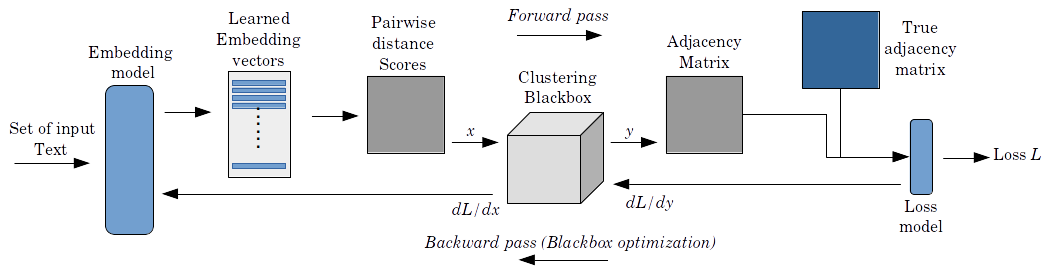
\includegraphics[scale=0.58]{acl-ijcnlp2021-templates/bbcluster_arch.png}
    \caption{Training loop of our proposed supervised clustering approach.}
    \label{fig:bbc_arch}
\end{figure*}
\subsection{Optimizing for RAND index} Our goal is to train the representation model, $V_\phi$, such that the resulting clusters maximize a clustering evaluation metric of our choice. In this work, we focus on optimizing for RAND index, a widely used clustering metric, which measures the similarity between the generated clusters and the clustering ground truth. If $y^* \in Y$ be the ground truth partition or the ideal clustering of $\mathcal{P}$, then the clustering quality of a candidate cluster $\hat{y}$ is expressed in terms of RAND index (RI):
\begin{align*}
RI &= \frac{\parbox{0.8\linewidth}{No. of unordered data pairs that agrees between $y^*$ and $\hat{y}$}}{\binom{n}{2}}
\end{align*}
where %a = sample pairs that share a cluster both in $y^*$ and $\hat{y}, b=$ sample pairs that do not share a cluster both in $y^*$ and $\hat{y}$ and 
$n=$ total number of data samples.

%\begin{comment}
\begin{table}[t]
\begin{small}
\caption{Description of variables used in Figure \ref{fig:bbc_arch}.}
\begin{tabular}{p{0.1\linewidth}p{0.8\linewidth}}
\hline
Variable & Description \\ \hline
$\mathcal{P}$ & Set of documents to be clustered \\
$V_\phi$ & Embedding model with trainable parameters $\phi$ \\
$V_\phi(\mathcal{P})$ & Representation vectors of $\mathcal{P}$ obtained using $V_\phi$  \\
$D$ & Pairwise distance matrix of vectors in $V_\phi(\mathcal{P})$ \\
$A$ & Adjacency matrix denoting clustering result \\
$T$ & Adjacency matrix denoting ground truth clusters
\end{tabular}
\label{tab:bbc_arch}
\end{small}
\end{table}
%\end{comment}
\subsection{COB Training Loop}
Figure \ref{fig:bbc_arch} and Table \ref{tab:bbc_arch} presents the overall training approach. The focus of the training loop is to train the representation model $V_\phi$. First, the set of representation vectors $V_\phi(\mathcal{P})$ is obtained for all documents in set $\mathcal{P}$. Then we encode the input to the clustering algorithm as a square symmetric matrix $D$ with pairwise Euclidean distance scores between vectors in $V_\phi(\mathcal{P})$. 
%For brevity, we simply use $V$ to denote the set of all embedding vectors, $V_\phi(\mathcal{P})$, from here on.
\begin{align*}
D_{ij} = ||V_\phi(p_i) - V_\phi(p_j)||_2 \quad \textrm{where} \quad p_i,p_j \in \mathcal{P}    
\end{align*}
The solution to the clustering problem is expressed in form of an adjacency matrix $A$ such that
\begin{align*}
A_{ij} = 1 \textrm{ if } i,j \textrm{ share same cluster and } 0 \textrm{ otherwise}    
\end{align*}
We denote the adjacency matrix of the clustering ground truth as $T$. Now, we can express RI using the following form:
\begin{align*}
    RI=1-\frac{\sum_{ij} |A_{ij}-T_{ij}|}{2\binom{n}{2}} \quad \textrm{see Appendix}
\end{align*}
It is clear from the above equation that if we want to maximize RI, we need to minimize the difference between $A$ and $T$. Intuitively, if we are able to produce ideal clustering results, then $A$ and $T$ would be identical, meaning $A-T$ is a zero matrix. Hence, we define our loss function $\mathcal{L}$ as the sum of $A-T$. Formally:
\begin{align*}
\mathcal{L} &= \sum_{ij}|A_{ij}-T_{ij}| 
%&=\sum_{i,j} A_{i,j}(1-T_{i,j}) + T_{i,j}(1-A_{i,j})
\end{align*}
The backward pass of this training loop involves estimating the gradient of the loss $\mathcal{L}$ with respect to the distance matrix $D$, the input to the clustering algorithm. This is achieved using blackbox backpropagation technique and the resulting gradient is used to drive a gradient descent algorithm for training the representation model $V_\phi$. 

\subsection{Regularization}\label{sec:reg} The purpose of any clustering algorithm is to identify groups of similar data points. By optimizing for a clustering metric such as RI, we learn a notion of similarity that most likely yields the ground truth clusters when used in HAC. However, we want to encourage a large margin between similar and dissimilar data points.
%we need to train the embedding model in such a way that it projects similar data points close to each other and dissimilar data points far apart. 
This is achieved when the loss function encourages \textit{inter-cluster} distances to increase and \textit{intra-cluster} distances to decrease. 
While this is part of the optimization process within the clustering algorithm, it is opaque during neural network training, due to the blackbox optimization technique. The clustering evaluation metric does not encourage a margin that is larger than necessary. 
%Although, the HAC algorithm optimizes for similar criterion, it is separate from our training loop as we treat the clustering component as a \textit{black box}. Hence, this is incorporated into the loss function by introducing a regularizer as described below.
Hence we incorporate a measure of intra versus inter-cluster distance as a regularizer in our optimization criterion as described below.
% If we so not include such criterion in the loss function then the model will not learn to distinguish between similar and dissimilar data enough because two clustering results may have the same ARI whether or not the similar elements are enough far apart from the dissimilar or not. But the learned model will be prone to make mistakes for unseen clustering data. Hence, it is necessary to enforce distinguishing power along with optimizing for RI.

\begin{align*}
    \mathcal{L}_{r} &= \mathcal{L} + r \cdot [\textrm{mean intra-cluster distance}\\ &- \textrm{mean inter-cluster distance}] \\
    &= \mathcal{L} + r \cdot \Bigg[\underbrace{\frac{\sum_{ij} D_{ij}T_{ij}}{\sum_{ij} T_{ij}}}_{\text{intra-cluster}} - \underbrace{\frac{\sum_{ij} D_{ij}(1-T_{ij})}{\sum_{ij}(1-T_{ij})}}_{\text{inter-cluster}}\Bigg] \\
    &\textrm{where $r$ is the regularization constant}
\end{align*}
The regularization constant $r$ controls how much emphasis is placed on increasing the margin between similar and dissimilar data points versus optimizing the clustering evaluation metric.

\section{Experimental Results}
In this section, we describe the datasets used for our experiments, discuss our evaluation paradigm and present experimental results that demonstrate efficacy of the representation model trained using our proposed training strategy over our baseline models.

\subsection{Datasets} To evaluate our proposed approach, we use two publicly available datasets: 20 newsgroups (20NG\footnote{Part of scikit-learn datasets~\citet{scikit-learn}}) and TREC Complex Answer Retrieval (CAR\footnote{\url{http://trec-car.cs.unh.edu/}}). As discussed earlier, for our proposed method, each training example consists of the ideal clustering of a set of documents. To produce enough such training samples, we choose to train and evaluate on multiple smaller clustering instances instead of a single but large clustering instance. We note that it will not make any difference in the way our baseline model is trained because they consume the training data in form of triples (SBERT Triplet), as long as we ensure that all models are trained on the same set of clustering examples. We take the following approach to construct such clustering benchmarks from the datasets (detailed statistics are presented in Table \ref{tab:dat20ng}):

\textbf{20NG dataset} is a widely used public collection of $18846$ documents, each categorized into any one of twenty topics. To convert this to a clustering benchmark, both train and test split of 20NG dataset is randomly grouped into sets of 50 documents along with their topic labels, resulting in 226 and 150 clustering instances respectively. Each set of 50 documents represents a single instance of clustering problem.
%Random sets of 50 documents each, along with their topic labels, are extracted from train and test split. Each of these sets represent a single instance of clustering problem. 
\begin{table}[t]
\begin{small}
\caption{Dataset statistics: $N=$ total no. of documents, $C=$ total no. of clustering instances, $n=$ average number of documents per clustering instance, $k=$ average number of clusters per clustering instance.}
\begin{tabular}{p{0.18\linewidth}p{0.08\linewidth}p{0.08\linewidth}p{0.08\linewidth}p{0.13\linewidth}p{0.13\linewidth}}
\hline
Dataset & N & C & n & k & \\ \hline
20NG train & 11314 & 226 & 50 & 18 & \\
20NG test  & 7532 & 150 & 50 & 18 & \\ \hline
&&&& k(coarse) & k(fine) \\ \hline
CAR train  & 6.8M & 597K & 11 & 3.84 & 5.04 \\
CAR test   & 6K & 126 & 47 & 7.78 & 17.16  
\end{tabular}
\label{tab:dat20ng}
\end{small}
\end{table}

\textbf{CAR dataset} (version $2.0$ year 1) is a large collection of Wikipedia articles. Each article consists of text passages about a topic, segmented into hierarchical subtopics using sections. From the CAR dataset, we use \texttt{train.v2.0} as train split (CAR train) and \texttt{benchmarkY1test} as test split (CAR test).  This dataset is originally designed for a passage retrieval task where passages in CAR articles are relevant for different sections under the overarching topic of the article. This relevance information is part of the dataset in form of the ground truth. We assume that all relevant passages for an article are already retrieved and our focus is to cluster these passages. So each article is a separate clustering problem where our task is to cluster all the passages of the article such that passages from same sections in the original article share the same cluster. We treat the section label under which a passage appears as the clustering label of the passage.

\begin{figure}[t]
    \centering
    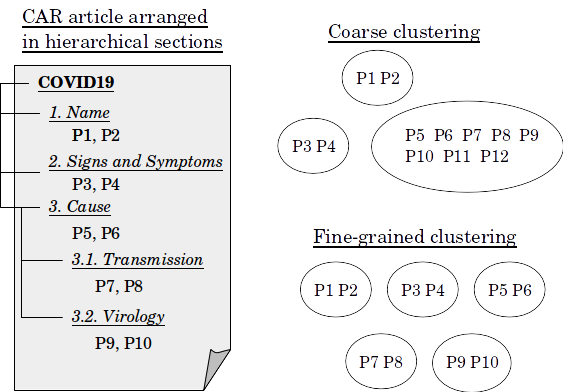
\includegraphics[scale=0.5]{acl-ijcnlp2021-templates/wiki_articles.png}
    \caption{Coarse and fine-grained clustering benchmarks from CAR dataset.}
    \label{fig:wiki}
\end{figure}

Section labels in CAR dataset are hierarchical. This provides an opportunity to evaluate our clustering models under different levels of granularity. As depicted in Figure \ref{fig:wiki}, passages $p_6$ and $p_7$ in article \textit{COVID 19}  belong to the sections \textit{Cause} and \textit{Cause/Transmission} respectively. For a coarse-grained view of the clustering, we consider $p_6,p_7$ under the same topic cluster \textit{Cause}. However, for fine-grained clustering we have to consider $p_6,p_7$ under separate subtopic clusters. The CAR dataset provides both in form of \textit{top-level} (coarse) and \textit{hierarchical} (fine-grained) benchmarks. We train and evaluate our models on both flavors of the dataset.

\begin{comment}
\begin{table}[t]
\begin{small}
\caption{Dataset statistics: $N,C,n,k$ denotes the same as Table \ref{tab:dat20ng}. Here, each clustering instance is a set of passages relevant for an article in Wikipedia.}
\begin{tabular}{lllllr}
\hline
Dataset & N & C & n & $k_{coarse}$ & $k_{fine}$ \\ \hline
CAR train  & 6.8M & 597K & 11 & 3.84 & 5.04 \\
CAR test   & 6K & 126 & 47 & 7.78 & 17.16   
\end{tabular}
\label{tab:dat}
\end{small}
\end{table}
\end{comment}

\subsection{Evaluation Paradigm} Our primary focus is to evaluate the efficacy of our proposed training strategy for supervised clustering and compare it with other training methods while ensuring the fairness of our evaluation. Hence, we train the same text embedding model with the same training data differing only in the training strategies. For the embedding model, we use Sentence-BERT~\citep{reimers2019sentence}, a recent BERT-based embedding model. Finally, macro-average performance on all clustering instances on the test sets are reported with statistical significance testing. We use three clustering evaluation metrics, RAND index (RI), Adjusted RAND index (ARI) and Normalized Mutual Information (NMI).

\paragraph{Compared methods.} In this section we discuss all the methods which are compared in our experiments. All methods are trained until no significant improvement is observed on the validation set. For each method, models are saved on regular interval and we use the best model found during training in terms of validation ARI score to evaluate on the test set.

\textbf{SBERT COB.} We train Sentence-BERT with our proposed training strategy and refer the obtained model as \textbf{SBERT COB}.

\textbf{SBERT Triplet.} To compare our approach with a strong supervised baseline, we train Sentence-BERT with Triplet loss function~\citep{dor2018learning}. It is designed to generate document representations that capture topical similarities. Here, each training example consists of two similar ($d,d^+$) and one dissimilar ($d^-$) documents. Triplet loss trains the document representation model $V_{trip}$ so that the Euclidean distance between the similar pair of representations $||V_{trip}(d)-V_{trip}(d^+)||_2$ is less than the negative pair $||V_{trip}(d)-V_{trip}(d^-)||_2$ by at least a margin $\epsilon$.

\begin{align*}
    \mathcal{L}_{triplet} &= \max(0, ||V_{trip}(d)-V_{trip}(d^+)||_2 \\
    & \quad -||V_{trip}(d)-V_{trip}(d^-)||_2+\epsilon)
\end{align*}

%\textbf{SBERT Binary} Similar to SBERT-Triplet except the Triplet loss is replaced by Binary loss. Inspired from works in image clustering~\citet{chang2017deep}, Binary loss simplifies the clustering process as a binary classification problem where each training sample consists of a pair of similar or dissimilar data points.

\textbf{Unsupervised baselines.} To compare the performances of unsupervised clustering approaches for our use cases, we also include:
\begin{enumerate}
\item \textit{SBERT raw}, the pre-trained Sentence-BERT model without any finetuning and
\item \textit{TFIDF} with cosine similarity as a more canonical approach.
\end{enumerate}

\subsection{Hyperparameter Optimization} The interpolation parameter $\lambda$ (Section \ref{sec:bb}) and regularization constant $r$ (Section \ref{sec:reg}) are two hyperparameters we have to tune in SBERT COB. We use Optuna~\citep{optuna_2019}, a recently proposed hyperparameter optimization framework, to search for optimum $\lambda, r$ pair in terms of validation performance for each dataset. Table \ref{tab:hyp} presents the optimum hyperparameter values used for our experiments.

\begin{table}[t]
\begin{small}
\caption{Optimum values for interpolation parameter $\lambda$ and regularization constant $r$ found using Optuna.}
\label{tab:hyp}
\begin{tabular}{p{0.55\linewidth}p{0.15\linewidth}p{0.15\linewidth}}
\hline
Dataset        & $\lambda$ & $r$ \\ \hline
NG20     & 90.0 & 1.0 \\
CAR coarse & 47.0 & 3.8 \\
CAR fine-grained & 103.0 & 0.3 
\end{tabular}
\end{small}
\end{table}

\subsection{Clustering Evaluation} Here we present details of all the experiments carried out and discuss the results. All experiments are executed on a single NVIDIA Titan XP GPU with 12GB memory. For all the SBERT models, we use uncased DistilBERT~\citep{sanh2019distilbert} as the underlying BERT embedding model.

\begin{table}[t]
\begin{small}
\caption{Clustering performance on NG20 dataset in terms of mean RAND index (RI), its corrected for chance version Adjusted RAND Index (ARI) and mean Normalized Mutual Information (NMI). Paired t-test ($\alpha=0.05$) is carried out with respect to SBERT Triplet (denoted with *) and $\blacktriangle$ and $\blacktriangledown$ denotes significantly higher or lower performance.}
\label{tab:ng20exp}
\begin{tabular}{p{0.35\linewidth}p{0.15\linewidth}p{0.15\linewidth}p{0.15\linewidth}}
\hline
Method        & RI & ARI & NMI \\ \hline
SBERT COB     & \textbf{0.925} & \textbf{0.233}$\blacktriangle$ & \textbf{0.725}$\blacktriangle$ \\
SBERT Triplet* & 0.924 & 0.223 & 0.721 \\
SBERT raw           & 0.754$\blacktriangledown$ & 0.041$\blacktriangledown$ & 0.582$\blacktriangledown$ \\
TFIDF         & 0.624$\blacktriangledown$ & 0.008$\blacktriangledown$ & 0.506$\blacktriangledown$ \\
\end{tabular}
\end{small}
\end{table}
\subsubsection{Experiment 1: 20NG} We train SBERT COB and other supervised methods using $80\%$ of the train split of 20NG dataset and the remainder is held out for validation. Table \ref{tab:ng20exp} presents the performance on the test set evaluated using mean RI, ARI and NMI.

We observe that our proposed method SBERT COB outperforms all other baselines in terms of RI, ARI and NMI. For ARI and NMI, the improvement is statistically significant in terms of paired t-test with $\alpha=0.05$ carried out with respect to the best performing baseline, SBERT Triplet. Both TFIDF and SBERT raw fail to obtain meaningful clusters, demonstrating the efficacy of supervised representation models in clustering context.

\subsubsection{Experiment 2: CAR} Due to large size of the CAR training split (\texttt{train.v2.0}), it is impractical to train SBERT Triplet with all possible triplets in the training set. Instead, we compare the supervised models trained on three smaller subsets of the training dataset. Each subset contains articles with exactly $n$ passages where $n=30, 35$ and $40$. However, they are always evaluated on the same CAR test set. These values of $n$ are chosen so that we obtain reasonable numbers of training samples while their statistics remain close to the CAR test set on which we are evaluating. Table \ref{tab:datsplit} presents statistics about these three training subsets. 

\begin{table}[t]
\begin{small}
\caption{Dataset statistics: $N,C,n,k$ denotes the same as Table \ref{tab:dat20ng}, $t$ denotes the total number of available triples to train SBERT Triplet method.}
\label{tab:datsplit}
\begin{tabular}%
{>{\raggedleft\arraybackslash}p{0.08\linewidth}%
>{\raggedleft\arraybackslash}p{0.05\linewidth}%
>{\raggedleft\arraybackslash}p{0.05\linewidth}%
>{\raggedleft\arraybackslash}p{0.11\linewidth}%
>{\raggedleft\arraybackslash}p{0.11\linewidth}%
>{\raggedleft\arraybackslash}p{0.11\linewidth}%
>{\raggedleft\arraybackslash}p{0.11\linewidth}%
}
\hline
%\multicolumn{1}{c}{Subset} & \multicolumn{1}{c}{N} & \multicolumn{1}{c}{C} & \multicolumn{1}{c}{$k_{coarse}$} & \multicolumn{1}{c}{$k_{fine}$} & \multicolumn{1}{c}{$t_{coarse}$} & \multicolumn{1}{c}{$t_{fine}$}  \\ \hline
Subset & N & C & k(coarse) & k(fine) & t(coarse) & t(fine) \\ \hline
%n=30 & 71280 & 2376 & 5.97 & 10.64 & 8.6M & 5.8M \\
%n=35 & 56175 & 1605 & 6.27 & 12.17 & 9.3M & 5.9M \\
%n=40 & 49920 & 1248 & 6.73 & 13.62 & 10.8M & 6.5M  
n=30 & 71K & 2.4K & 5.97 & 10.64 & 8.6M & 5.8M \\
n=35 & 56K & 1.6K & 6.27 & 12.17 & 9.3M & 5.9M \\
n=40 & 50K & 1.2K & 6.73 & 13.62 & 10.8M & 6.5M
\end{tabular}
\end{small}
\end{table}

\begin{figure}[t]
    \centering
    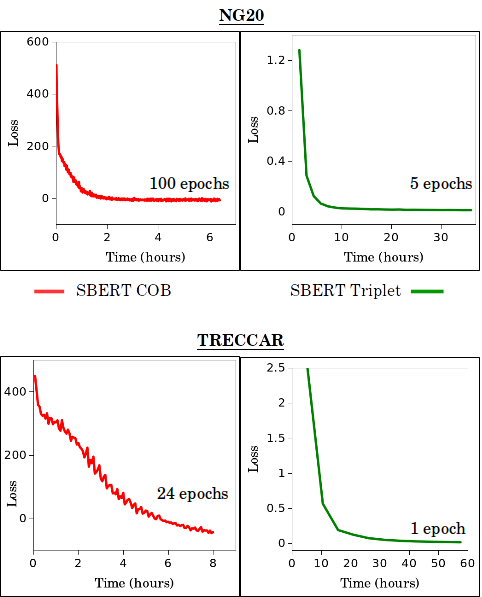
\includegraphics[scale=0.6]{acl-ijcnlp2021-templates/training_loss3.png}
    \caption{Comparison between SBERT COB and SBERT Triplet in terms of total training time.}
    \label{fig:train}
\end{figure}

\begin{table}[h]
\begin{small}
\caption{Coarse-level clustering performance on CAR dataset using top-level benchmarks. Supervised models are trained with set of clustering examples each containing $n$ passages. Paired t-test ($\alpha=0.05$) is carried out with respect to SBERT Triplet ($n=30$) and marked with *.}
\label{tab:trecexp}
\begin{tabular}{p{0.4\linewidth}p{0.12\linewidth}p{0.12\linewidth}p{0.12\linewidth}}
\hline
Method        & RI & ARI & NMI \\ \hline
%SBERT Binary  &          &          \\
Trained on n=30 subset&&\\
SBERT COB     & 0.742 & 0.230 & 0.502 \\
SBERT Triplet* & 0.738 & 0.214 & 0.494 \\ \hline
%DBC           & 0.075$\blacktriangledown$ & 0.375$\blacktriangledown$ \\ \hline
Trained on n=35 subset&&\\
SBERT COB     & \textbf{0.744} & \textbf{0.236} & 0.512$\blacktriangle$ \\
SBERT Triplet & 0.715$\blacktriangledown$ & 0.167$\blacktriangledown$ & 0.460$\blacktriangledown$ \\ \hline
%DBC           & 0.069$\blacktriangledown$ & 0.367$\blacktriangledown$ \\ \hline
Trained on n=40 subset&&\\
SBERT COB     & 0.726 & 0.231 & \textbf{0.514}$\blacktriangle$ \\
SBERT Triplet & 0.704$\blacktriangledown$ & 0.145$\blacktriangledown$ & 0.438$\blacktriangledown$ \\ \hline
%DBC           & 0.036$\blacktriangledown$ & 0.330$\blacktriangledown$ \\ \hline
Unsupervised&&\\
SBERT raw & 0.563$\blacktriangledown$ & 0.101$\blacktriangledown$ & 0.406$\blacktriangledown$ \\
TFIDF         & 0.544$\blacktriangledown$ & 0.072$\blacktriangledown$ & 0.375$\blacktriangledown$
\end{tabular}
\end{small}
\end{table}

\begin{table}[h]
\begin{small}
\caption{Fine-grained clustering performance on CAR dataset using hierarchical benchmarks. Notations used are same as in Table \ref{tab:trecexp}.}
\label{tab:trecexp2}
\begin{tabular}{p{0.4\linewidth}p{0.12\linewidth}p{0.12\linewidth}p{0.12\linewidth}}
\hline
Method        & RI & ARI & NMI \\ \hline
%SBERT Binary  &          &          \\
Trained on n=30 subset&&\\
SBERT COB     & 0.849 & \textbf{0.178} & \textbf{0.682} \\
SBERT Triplet* & 0.848 & 0.173 & 0.678 \\ \hline
%DBC           & 0.089$\blacktriangledown$ & 0.607$\blacktriangledown$ \\ \hline
Trained on n=35 subset&&\\
SBERT COB     & 0.837$\blacktriangledown$ & 0.163 & 0.672 \\
SBERT Triplet & 0.830$\blacktriangledown$ & 0.152$\blacktriangledown$ & 0.665$\blacktriangledown$ \\ \hline
%DBC           & 0.077$\blacktriangledown$ & 0.595$\blacktriangledown$ \\ \hline
Trained on n=40 subset&&\\
SBERT COB     & 0.832$\blacktriangledown$ & 0.154 & 0.666$\blacktriangledown$ \\
SBERT Triplet & \textbf{0.860}$\blacktriangle$ & 0.138$\blacktriangledown$ & 0.662$\blacktriangledown$ \\ \hline
%DBC           & 0.066$\blacktriangledown$ & 0.582$\blacktriangledown$ \\ \hline
Unsupervised&&\\
SBERT raw & 0.796$\blacktriangledown$ & 0.130$\blacktriangledown$ & 0.646$\blacktriangledown$ \\
TFIDF         & 0.788$\blacktriangledown$ & 0.110$\blacktriangledown$ & 0.631$\blacktriangledown$
\end{tabular}
\end{small}
\end{table}

\begin{figure*}[h]
    \centering
    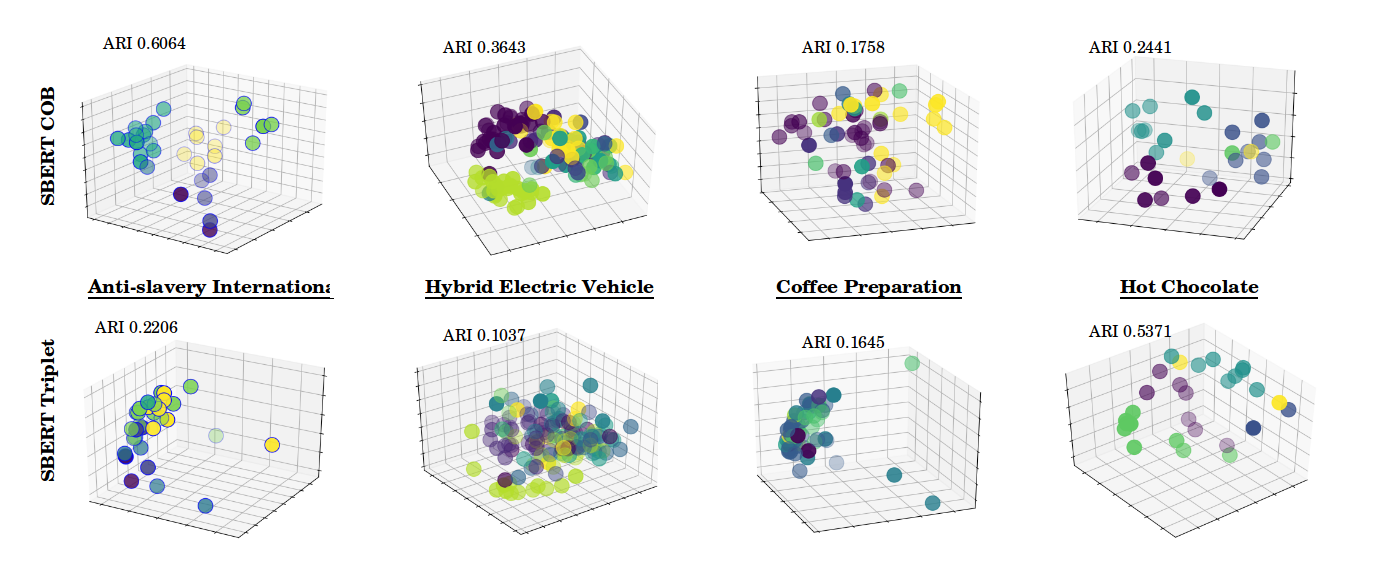
\includegraphics[scale=0.45]{acl-ijcnlp2021-templates/compare_cluster_viz.png}
    \caption{Visual comparison of clustering results between SBERT COB and SBERT Triplet ($n=35$). Each dot denotes a passage from an article projected into the representation space after applying PCA. Different color denotes different subtopics. Clear separation of different colored blobs indicates good clustering quality. }
    \label{fig:viz}
\end{figure*}

We report the coarse and fine-grained clustering performance in Table \ref{tab:trecexp} and Table \ref{tab:trecexp2} respectively. For both coarse and fine-grained clustering, we observe that for each of the training splits ($n=30,35,40$), our proposed method SBERT COB consistently performs better than the best performing baseline, SBERT Triplet ($n=30$) in terms of both ARI and NMI. As expected, clustering performance in terms of RI score mostly correlates with ARI score. The only exception is SBERT Triplet trained on $n=40$ for fine-grained clustering.  However, we also observe overall decrease in ARI scores for all methods in case of fine-grained clustering. This is expected as fine-grained clustering is a harder problem largely due to fewer passage pairs sharing a cluster. Note that RI and NMI measures are only comparable within table because unlike ARI, it is not adjusted for chance.

\subsubsection{Experiment 3: Training Convergence} 
Existing methods for learning clustering representation spaces, focus solely on classifying individual pairs as similar or different, and hence ignore to which extent other data points already form clusters. The key difference in our work is that we learn the representation space to directly optimize for the clustering evaluation metric, which is based on the clustering results of HAC when used with pairwise Euclidean distances. This allows the model to reach convergence much faster, leading to reduced overall training time, when compared to other methods that uses only a sub-sample of each clustering example (e.g. Triplets). This is particularly helpful in scenarios when we want to regularly update our model to incorporate new training examples.

To demonstrate this we present Figure \ref{fig:train} that compares the time taken to reach convergence during training of SBERT Triplet and SBERT COB on 20NG dataset and CAR dataset (coarse $n=35$) respectively. For both the datasets, SBERT COB is able to converge at least five times sooner than SBERT Triplet, leading to much faster overall training time. Moreover, for NG20 dataset each epoch of SBERT COB is about 100 times faster than SBERT Triplet. This leads to decrease in overall training time even though SBERT COB takes many more epochs to converge than SBERT Triplet. We observe similar training behaviour for CAR dataset.
%As SBERT Triplet is agnostic to the overall clustering performance of the trained model, it converges quickly after optimizing a relaxed version of the clustering problem, the triplet loss. But SBERT COB has a more complex loss landscape to explore that results in slow convergence in terms of number of iterations but allows it to learn more accurate representation of the clustering solution. Here we want to also emphasize that a single iteration of SBERT COB is much faster than the same of SBERT Triplet as reported in figure. Due to this, SBERT COB is able to reach convergence much faster than SBERT Triplet in terms of time in hours. We observe similar results on TRECCAR dataset.

%\subsection{Overfitting on TRECCAR dataset} Unlike NG20, we observe that both the models suffer from overfitting according to the validation performance on both flavors of the TRECCAR dataset. Note here that each clustering instance in NG20 is a sample of documents drawn from the same distribution of twenty topics. But for TRECCAR, each clustering instance is a set of passages relevant for a specific topic in Wikipedia. This is why it is difficult to learn a generalized clustering model for TRECCAR dataset. Despite the fact, SBERT COB is able to consistently achieve high ARI scores on the test set as demonstrated earlier suggesting that SBERT COB is able to generalize better than SBERT Triplet.

\subsection{Qualitative Evaluation} Here, we demonstrate efficacy of SBERT COB over SBERT Triplet ($n=35$) through visual comparison of clustering results from the CAR dataset. Principle Component Analysis (PCA) is used to transform the representation vectors into 3D vectors which are then visualized as points in 3D vector space. Figure \ref{fig:viz} compares the results obtained for four articles from CAR test split.

For articles \textit{Anti-slavery International} and \textit{Hybrid Electric Vehicle}, SBERT COB is able to clearly identify clusters of different topics and projects them in different regions of the embedding space. On the contrary, it is difficult to find any clear cluster boundaries in the SBERT Triplet representation space which is also reflected in the ARI scores obtained by the methods. For the article \textit{Coffee Preparation}, both the methods perform poorly in terms of ARI scores. But in case of SBERT COB we see a tendency to separate dissimilar passages. SBERT Triplet projects almost all the passages in a dense region except for a few outlier passages. For the article \textit{Hot Chocolate}, SBERT Triplet obtains numerous small clusters of similar passages. As ARI metric is based on sample-pairs, SBERT Triplet obtains better ARI score even though it does not achieve clear groupings of similar elements.

It is clear from the examples that SBERT COB provides better global clustering quality than SBERT Triplet. This is expected because unlike SBERT Triplet, SBERT COB observes the relationships between all passages in a clustering instance at once to directly optimize for RAND index. Hence, SBERT COB is able to make better global clustering decisions than other pair-based methods. %Although sometimes it fools ARI, but visually SBERT COB is better

\subsection{Quadratic Scaling of SBERT COB} As SBERT COB learns from all possible interactions of data points in a clustering instance at once, it requires all the adjacency matrices in a batch of clustering samples to fit in memory. Thus the space complexity increases quadratically with the size of each clustering instance. Hence, the batch size is kept small to allow training with a limited GPU memory. However, even with batch size of 1, SBERT COB is observed to obtain superior results in terms of training speed and clustering performance as reported earlier.

\section{Conclusion} In this work, we propose an alternative training strategy to train a representation model, for clustering. Our training strategy, COB (Clustering Optimization as Blackbox), directly optimizes the RAND index, a clustering evaluation metric. Using our method, we train SBERT COB, a BERT-based text representation model. We empirically show that SBERT COB significantly outperforms other supervised and unsupervised text embedding model on two separate datasets in terms of RI, ARI and NMI, indicating better cluster quality. Visual representations of the resulting vectors also confirm that SBERT COB learns to holistically distinguish clusters of different topics. Moreover, each epoch in SBERT COB training loop is about 100 times faster when compared to SBERT Triplet, our best performing baseline method. This leads to a significant decrease in overall training time even though SBERT COB requires more iterations to converge than SBERT Triplet. This makes SBERT COB suitable for applications that require clustering models to be updated on a regular basis as new training samples become available. Lastly, although we have conducted experiments with a specific clustering algorithm (HAC) and a clustering metric to optimize (RAND index), our model is independent of the particular choice of algorithm or the metric.

\bibliographystyle{acl_natbib}
\bibliography{acl2021}

\appendix 

\section{Relation between RAND index and Adjacency matrix} Given a set of $n$ data points $\mathcal{P}$, let us compare two clustering results of $\mathcal{P}$, $C_T$ and $C_A$, in terms of RAND index. We know that RAND index is expressed as:
\begin{align*}
    RI &= \frac{a+b}{\binom{n}{2}} \\
    \textrm{where } a &= \textrm{number of pairs that share the same} \\ 
    & \quad \textrm{cluster both in $C_T$ and $C_A$} \\
    \textrm{where } b &= \textrm{number of pairs that are from different} \\
    & \quad \textrm{clusters both in $C_T$ and $C_A$}
\end{align*}

\begin{figure}[t]
    \centering
    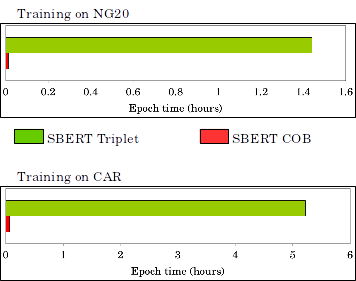
\includegraphics[scale=0.75]{acl-ijcnlp2021-templates/epoch_time.png}
    \caption{Comparison between SBERT COB and SBERT Triplet in terms of epoch time.}
    \label{fig:train}
\end{figure}
Now we can express any clustering result $C_M$ in form of an adjacency matrix $M$ where $M_{ij}=1$ if the $i,j$-th data points in $\mathcal{P}$ share the same cluster in $C_M$ and $M_{ij}=0$ otherwise. We represent the clustering results $C_T$ and $C_A$ with such adjacency matrices $T$ and $A$ respectively. Also, the difference matrix of $A,T$ denoted as $|A-T|$ indicates the ordered pairs that do not agree between $A,T$. In other words, $|A_{ij}-T_{ij}|=1$ denotes that the $i,j$-th data points do not agree between $A$ and $T$. Now, we can express RAND index in terms of $A$ and $T$ as follows:

\begin{align*}
    RI &= \frac{a+b}{\binom{n}{2}} \\
    &= \frac{\text{No. of agreements between } C_T,C_A}{\binom{n}{2}} \\
    &= \frac{\parbox{0.9\linewidth}{No. of unordered pairs in $\mathcal{P}$ that agrees between $C_T,C_A$}}{\binom{n}{2}} \\
    &= \frac{\parbox{0.9\linewidth}{No. of ordered pairs in $\mathcal{P}$ that agrees between $C_T,C_A$}}{2\binom{n}{2}} \\
    &= \frac{\text{Total ordered pairs in $\mathcal{P}$}-\sum_{ij} |A_{ij}-T_{ij}|}{2\binom{n}{2}} \\
    &= \frac{2\binom{n}{2}-\sum_{ij} |A_{ij}-T_{ij}|}{2\binom{n}{2}} \\
    &= 1-\frac{\sum_{ij} |A_{ij}-T_{ij}|}{2\binom{n}{2}}
\end{align*}

\section{Comparison of Epoch Time} 
Figure \ref{fig:train} shows the mean epoch time of SBERT Triplet and SBERT COB on 20NG dataset and CAR dataset (coarse n = 35) respectively.

\end{document}
